\documentclass[convert={density=300,size=1080x800,outext=.png}]{standalone}
\usepackage{tikz}
\usetikzlibrary{positioning, matrix, arrows}

\thispagestyle{empty}

\begin{document}
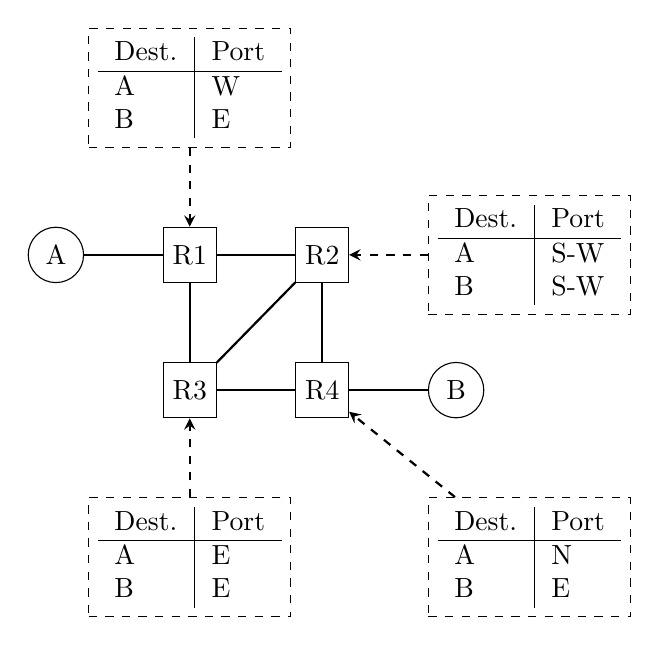
\begin{tikzpicture}

\tikzstyle{arrow} = [thick,->,>=stealth]
\tikzset{router/.style = {rectangle, draw, text centered, minimum height=2em}, }
\tikzset{host/.style = {circle, draw, text centered, minimum height=2em}, }
\tikzset{ftable/.style={rectangle, dashed, draw} }
\node[host] (A) {A};
\node[router, right=of A] (R1) { R1 };
\node[ftable, above=of R1] (FR1) { \begin{tabular}{l|l} 
		Dest. & Port \\
		\hline 
		A & W \\
		B & E \\
\end{tabular}};
\node[router,right=of R1] (R2) {R2};
\node[ftable, right=of R2] (FR2) { \begin{tabular}{l|l} 
		Dest. & Port \\
		\hline 
		A & S-W \\
		B & S-W \\
	\end{tabular}\\};
\node[router,below=of R1] (R3) {R3};
\node[ftable, below=of R3] (FR3) { \begin{tabular}{l|l} 
		Dest. & Port \\
		\hline 
		A & E \\
		B & E \\
	\end{tabular}\\};
\node[router,below=of R2] (R4) {R4};
\node[ftable, below right=of R4] (FR4) { \begin{tabular}{l|l} 
		Dest. & Port \\
		\hline 
		A & N \\
		B & E \\
	\end{tabular}\\};
\node[host, right=of R4] (B) {B};

\path[draw,thick]
(A) edge (R1) 
(R1) edge (R2) 
(R2) edge (R3) 
(R1) edge (R3) 
(R4) edge (R3) 
(R2) edge (R4) 
(R4) edge (B); 

\draw[arrow, dashed] (FR1) -- (R1); 
\draw[arrow, dashed] (FR2) -- (R2); 
\draw[arrow, dashed] (FR3) -- (R3); 
\draw[arrow, dashed] (FR4) -- (R4); 
\end{tikzpicture}
\end{document}
